
\chapter{Diagramme zeichnen}
\autor{Thomas Hilarius Meyer}

allgemeine vs. spezielle Lösungen

\section{Der unsaubere Weg: Open Office und co. benutzen}

Einbinden der fertigen Abb. als Grafik


\section{Die beiden wichtigsten Pakete: pstricks und tikz}

\minisec{pstricks}
\paket{pstricks}

\minisec{tikz}
\paket{tikz}

\section{Konkrete Anwendungen}


\subsection{Linguistische Strukturen}
\index{Linguistik} \index{x-bar-Schema} \index{Phrasenstruktur}
\paket{covington}
\footcite{roemer:dtk2008}
\footcite{roemer:dtk2016}


\subsection{Baumdiagramme}
\index{Baumdiagramm} \index{Stemma}

Das Paket \paket{forest} von Saso Zivanovic erlaubt einfache und sehr komplexe Baumsstrukturen:

\begin{lfgwexample}{}
 \begin{forest}
  [VP
    [DP]
    [V'
      [V]
      [DP]
    ]
  ]
\end{forest}
\end{lfgwexample}

\subsection{Stammbäume}

Mit \paket{forest} und den zahlreichen anderen Paketen zum Zeichnen mathematisch/linguistischer
Baumstrukturen stoßen Geisteswissenschaftler bei einem häufigen Anwendungsfall schnell an eine
Grenze:

Natürliche Stammbäume sind -- auch bei einfachsten familiären Strukturen -- stets mehrfach
verzweigt: Ein Vater und eine Mutter haben gemeinsame Kinder. 
In der historiographischen Realität müssen häufig noch wesentlich komplexere Familenstrukturen
abgebildet werden.

Für die Bedürfnisse von Historikern und Familenforschern wurde das Paket \paket{genealogytree}
von Thomas F. Sturm entwickelt.
Es bietet die Möglichkeit, praktisch beliebig komplexe Familienstrukturen als Stammbaum darzustellen;
das Aussehen der Stammbäume kann auf vielfältige Weise den eigenen Vorstellungen angepasst werden.
Das Paket ist ausgesprochen umfangreich und -- der Komplexität der Aufgabenstellung geschuldet --
seine Benutzung ist nicht ganz trivial.
Allerdings enthält es eine knapp 300-seitige, vorzügliche Dokumentation mit zahlreichen Beispielen,
mit deren Hilfe man reale Familienstrukturen  angehen kann:

Zunächst muss das Paket in der Präambel eingebunden werden:
\lstinline/\usepackage[all]{genealogytree}/.

Typische westliche Kleinfamilie:

\begin{lfgwexample}{}
    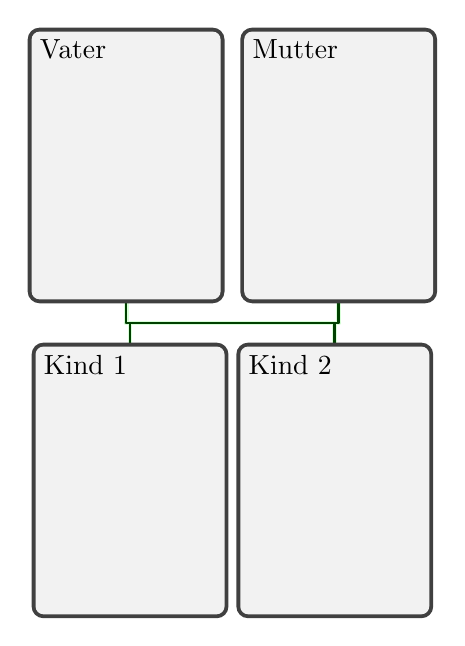
\begin{tikzpicture}
    \genealogytree{
        parent{
            p{Vater}
            p{Mutter}
            g{Kind 1}
            c{Kind 2}
        }
    }
    \end{tikzpicture}
\end{lfgwexample}



der Merowinger

\begin{lfgwcode}{}
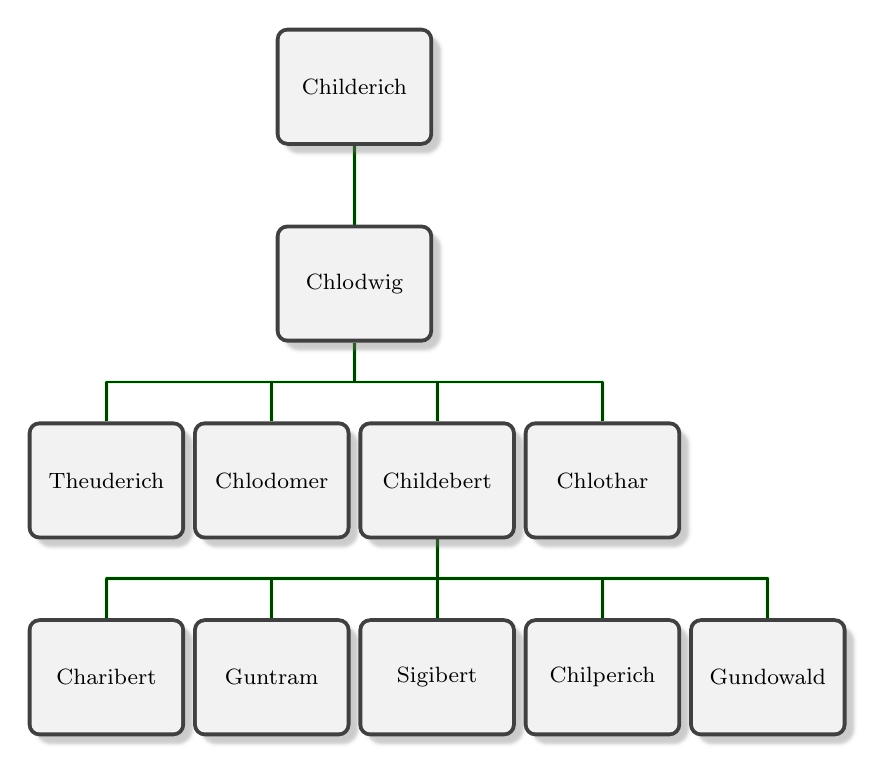
\begin{tikzpicture}
 \genealogytree[template=signpost]{
  parent{
    c{Charibert}
    c{Guntram}
    c{Sigibert}
    g{Chilperich}
    c{Gundowald}
    parent{
      c{Theuderich}
      c{Chlodomer}
      g{Childebert}
      c{Chlothar}
      parent{
        g{Chlodwig}
        parent{
          g{Childerich}
        }
      }
    } 
  }
}
\end{tikzpicture}
\end{lfgwcode}


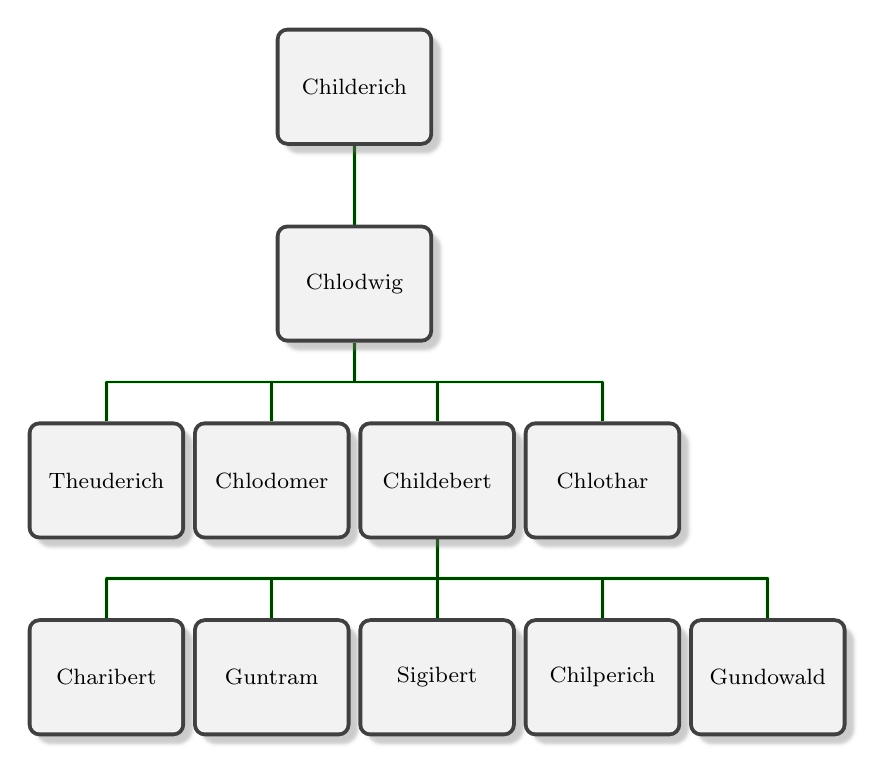
\begin{tikzpicture}
\genealogytree[template=signpost]{
    parent{
        c{Charibert}
        c{Guntram}
        c{Sigibert}
        g{Chilperich}
        c{Gundowald}
        parent{
            c{Theuderich}
            c{Chlodomer}
            g{Childebert}
            c{Chlothar}
            parent{
                g{Chlodwig}
                parent{
                    g{Childerich}
                }
            }
        } 
    }
}
\end{tikzpicture}

\subsection{Zeitschienen}

Das kleine Paket \paket{chronology} von Levi Wiseman eignet sich hervorragend, um ohne großen
Aufwand eine Zeitschiene zu erstellen.

\begin{lfgwexample}{}
 \begin{chronology}[5]{1930}{1950}{6cm}
     \event{1933}{Machtergreifung Hitlers}
     \event[1939]{1945}{Zweiter Weltkrieg}
 \end{chronology}
\end{lfgwexample}



\subsection{Statistiken visualisieren}

Torten- und Balkendiagramme... 

\paket{datatool} ?

\paket{pgf-pie} ist nur in Miktex enthalten; ansonsten problemlos nachinstallierbar von 
www.ctan.org (und Abspeichern im Arbeitsverzeichnis).

\begin{lfgwexample}{}
    \begin{tikzpicture}
       \pie[text=inside, sum=auto, after number=,]
           {44/DNVP, 
            4/Wirtschaftspartei,  
            19/DVP, 
            91/Zentrum,
            75/DDP,
            163/SPD,
            22/USPD,
            2/Sonstige}
    \end{tikzpicture}
\end{lfgwexample}

